\documentclass[aps,pra,12pt,nofootinbib,superscriptaddress,longbibliography,showpacs]{revtex4-1}

\usepackage[utf8]{inputenc}
\usepackage[T1]{fontenc}
\usepackage[english]{babel}  % english language

\usepackage{amssymb,amsmath,amsfonts,amsthm}
\usepackage{mathtools}
\usepackage{verbatim}
\usepackage{enumerate}
%\usepackage{tensor}
\usepackage{fancyhdr}
\pagestyle{fancy}
\usepackage{graphicx}
\graphicspath{{pics/}}
\usepackage{hyperref}
\usepackage{bbm}


\newcommand{\bydef}{\stackrel{\mathrm{def}}{=}}
\renewcommand{\baselinestretch}{1}  % cancels any possible double spacing

\usepackage{color}
%Some shortcuts added for edits
\definecolor{dred}{rgb}{.8,0.2,.2}
\definecolor{ddred}{rgb}{.8,0.5,.5}
\definecolor{dblue}{rgb}{.2,0.2,.8}
% suggested change
\newcommand{\add}[1]{\textcolor{dred}{*** #1 ***}} 
% suggested to remove
\newcommand{\out}[1]{\textcolor{ddred}{\textbf{[}\emph{#1}\textbf{]}}}
% comment or remark
\newcommand{\yo}[1]{\textcolor{dblue}{\textbf{[}#1\textbf{]}}}
\newcommand{\todo}[1]{\textbf{\underline{\textcolor{dblue}{\textbf{[}#1\textbf{]}}}}}

\theoremstyle{plain}
\newtheorem{theorem}{Theorem}   %[section]
\newtheorem{proposition}[theorem]{Proposition}
\newtheorem{lemma}[theorem]{Lemma}
\newtheorem{corollary}[theorem]{Corollary}

\theoremstyle{definition}
\newtheorem{definition}[theorem]{Definition}
\newtheorem{example}[theorem]{Example}
\newtheorem{remark}[theorem]{Remark}

% bra and ket: 
\newcommand{\bra}[1]{\mbox{$\langle #1|$}}
\newcommand{\ket}[1]{\ensuremath{|#1\rangle}}
\newcommand{\braket}[2]{\mbox{$\langle #1|#2\rangle$}}
\newcommand{\ketbra}[2]{\mbox{$|#1\rangle\langle #2|$}}
\newcommand{\iprod}[2]{\ensuremath{\langle #1,#2 \rangle}}

\newcommand{\gate}[1]{\ensuremath{\text{\sc #1}}}
\newcommand{\COPY}[1][]{\ensuremath{\gate{COPY}_{#1}}}

\newcommand{\comm}[2]{\ensuremath{\left[#1, #2\right]}}

\newcommand{\eq}{\Leftrightarrow}

\DeclareMathOperator{\Tr}{Tr}
\DeclareMathOperator{\Real}{Re}
\DeclareMathOperator{\Imag}{Im}
\DeclareMathOperator{\Span}{span}
\DeclareMathOperator{\diag}{diag}
\DeclareMathOperator{\Aut}{Aut} % automorphism group
\DeclareMathOperator{\End}{End} % set of endomorphisms

\newcommand{\projector}[1]{\mbox{$|#1\rangle\langle #1|$}}

\newcommand{\x}{\mathbf{x}}
\newcommand{\y}{\mathbf{y}}

\newcommand{\hprod}{\odot}

\newcommand{\I}{\openone}     % identity operator
\newcommand{\R}{{\mathbb R}}  % real numbers
%\newcommand{\C}{{\mathbb C}}  % complex numbers
\newcommand{\hilb}[1]{\ensuremath{\mathcal{#1}}} % Hilbert space
\newcommand{\swap}{{\sf{SWAP}}}
\newcommand{\ie}{i.e.}

% defines logic function names, to look nice 
\newcommand{\be}{\begin{equation}}
\newcommand{\ee}{\end{equation}}

\newcommand{\Figref}[1]{Figure \ref{#1}}

% Quantum communication, Formalism

\def\thesection{%
\arabic{section}}%
\def\thesubsection{%
\arabic{subsection}}%
\def\thesubsubsection{%
\arabic{subsubsection}}%
\def\theparagraph{%
\arabic{paragraph}}%
\def\thesubparagraph{%
\theparagraph.\arabic{subparagraph}}%
\setcounter{secnumdepth}{5}%

% please leave these here 


% fonts 
\def\1#1{{\bf #1}}
\def\2#1{{\cal #1}}
\def\7#1{{\mathbb #1}}


%-------------------------------------------
% Tomi's stuff
%-------------------------------------------

% Fractions
\newcommand{\half}{\mbox{$\textstyle \frac{1}{2}$}}
\newcommand{\quarter}{\mbox{$\textstyle \frac{1}{4}$}}

% Dirac notation
%\newcommand{\ket}[1]{\left | \, #1 \right \rangle}
\newcommand{\kets}[1]{ | \, #1 \rangle}
%\newcommand{\bra}[1]{\left \langle #1 \, \right |}
\newcommand{\bras}[1]{ \langle #1 \, \right}
%\newcommand{\braket}[2]{\left\langle\, #1\,|\,#2\,\right\rangle}
\newcommand{\brakets}[2]{\langle\, #1\,|\,#2\,\rangle}
\newcommand{\bracket}[3]{\left\langle #1 \left| #2 \right| #3 \right\rangle}
\newcommand{\brackets}[3]{\langle #1 | #2 | #3 \rangle}
\newcommand{\proj}[1]{\ket{#1}\bra{#1}}
\newcommand{\av}[1]{\langle #1\rangle}
\newcommand{\outprod}[2]{\ket{#1}\bra{#2}}

% Common operators
\newcommand{\tr}{\textrm{tr}}
%\newcommand{\Tr}{\mathrm{Tr}}
\newcommand{\od}[2]{\frac{\mathrm{d} #1}{\mathrm{d} #2}}
\newcommand{\pd}[2]{\frac{\partial #1}{\partial #2}}
\newcommand{\dt}[1]{\frac{\partial #1}{\partial t}}

% Second quantisation
\newcommand{\an}[1]{\hat{#1}}
\newcommand{\cre}[1]{\hat{#1}^\dag}
\newcommand{\vac}{\ket{\textrm{vac}}}

% Other quantum
\newcommand{\cc}{\textrm{c.c.}}

% Common letters
%\newcommand{\ee}{\mathrm{e}}
%\newcommand{\ii}{\mathrm{i}}
%\newcommand{\dd}{\mathrm{d}}
\newcommand{\identity}{\mathbbm{1}}

% Common symbols
\newcommand{\up}{\uparrow}
\newcommand{\down}{\downarrow}

\renewcommand{\Re}{\mathfrak{Re}}
\renewcommand{\Im}{\mathfrak{Im}}

% Letters in different styles

\newcommand{\AAA}{\mathbf{A}}
\renewcommand{\AA}{\mathcal{A}}
\newcommand{\aaa}{\mathbf{a}}
\renewcommand{\aa}{\mathrm{a}}
\newcommand{\BBB}{\mathbf{B}}
\newcommand{\BB}{\mathcal{B}}
\newcommand{\bbb}{\mathbf{b}}
\newcommand{\bb}{\mathrm{b}}
\newcommand{\CCC}{\mathbf{C}}
\newcommand{\CC}{\mathcal{C}}
\newcommand{\ccc}{\mathbf{c}}
\renewcommand{\cc}{\mathrm{c}}
\newcommand{\DDD}{\mathbf{D}}
\newcommand{\DD}{\mathcal{D}}
\newcommand{\ddd}{\mathbf{d}}
\newcommand{\dd}{\mathrm{d}}
\newcommand{\EEE}{\mathbf{E}}
\newcommand{\EE}{\mathcal{E}}
\newcommand{\eee}{\mathrm{e}}
%\newcommand{\ee}{\mathrm{e}}
\newcommand{\FFF}{\mathbf{F}}
\newcommand{\FF}{\mathcal{F}}
\newcommand{\fff}{\mathbf{f}}
\newcommand{\ff}{\mathrm{f}}
\newcommand{\GGG}{\mathbf{G}}
\newcommand{\GG}{\mathcal{G}}
\renewcommand{\ggg}{\mathbf{g}}
\renewcommand{\gg}{\mathrm{g}}
\newcommand{\HHH}{\mathbf{H}}
\newcommand{\HH}{\mathcal{H}}
\newcommand{\hhh}{\mathbf{h}}
\newcommand{\hh}{\mathrm{h}}
\newcommand{\III}{\mathbf{I}}
\newcommand{\II}{\mathcal{I}}
\newcommand{\iii}{\mathbf{i}}
\newcommand{\ii}{\mathrm{i}}
\newcommand{\JJJ}{\mathbf{J}}
\newcommand{\JJ}{\mathcal{J}}
\newcommand{\jjj}{\mathbf{j}}
\newcommand{\jj}{\mathrm{j}}
\newcommand{\KKK}{\mathbf{K}}
\newcommand{\KK}{\mathcal{K}}
\newcommand{\kkk}{\mathbf{k}}
\newcommand{\kk}{\mathrm{k}}
\newcommand{\LLL}{\mathbf{L}}
\newcommand{\LL}{\mathcal{L}}
\renewcommand{\lll}{\mathbf{l}}
\renewcommand{\ll}{\mathrm{l}}
\newcommand{\MMM}{\mathbf{M}}
\newcommand{\MM}{\mathcal{M}}
\newcommand{\mmm}{\mathbf{m}}
\newcommand{\mm}{\mathrm{m}}
\newcommand{\NNN}{\mathbf{N}}
\newcommand{\NN}{\mathcal{N}}
\newcommand{\nnn}{\mathbf{n}}
\newcommand{\nn}{\mathrm{n}}
\newcommand{\OOO}{\mathbf{O}}
\newcommand{\OO}{\mathcal{O}}
\newcommand{\ooo}{\mathbf{o}}
\newcommand{\oo}{\mathrm{o}}
\newcommand{\PPP}{\mathbf{P}}
\newcommand{\PP}{\mathcal{P}}
\newcommand{\ppp}{\mathbf{p}}
\newcommand{\pp}{\mathrm{p}}
\newcommand{\QQQ}{\mathbf{Q}}
\newcommand{\QQ}{\mathcal{Q}}
\newcommand{\qqq}{\mathbf{q}}
\newcommand{\qq}{\mathrm{q}}
\newcommand{\RRR}{\mathbf{R}}
\newcommand{\RR}{\mathcal{R}}
\newcommand{\rrr}{\mathbf{r}}
\newcommand{\rr}{\mathrm{r}}
\newcommand{\SSS}{\mathbf{S}}
\renewcommand{\SS}{\mathcal{S}}
\newcommand{\sss}{\mathbf{s}}
\renewcommand{\ss}{\mathrm{s}}
\newcommand{\TTT}{\mathbf{T}}
\newcommand{\TT}{\mathcal{T}}
\newcommand{\ttt}{\mathbf{t}}
\renewcommand{\tt}{\mathrm{t}}
\newcommand{\UUU}{\mathbf{U}}
\newcommand{\UU}{\mathcal{U}}
\newcommand{\uuu}{\mathbf{u}}
\newcommand{\uu}{\mathrm{u}}
\newcommand{\VVV}{\mathbf{V}}
\newcommand{\VV}{\mathcal{V}}
\newcommand{\vvv}{\mathbf{v}}
\newcommand{\vv}{\mathrm{v}}
\newcommand{\WWW}{\mathbf{W}}
\newcommand{\WW}{\mathcal{W}}
\newcommand{\www}{\mathbf{w}}
\newcommand{\ww}{\mathrm{w}}
\newcommand{\XXX}{\mathbf{X}}
\newcommand{\XX}{\mathcal{X}}
\newcommand{\xxx}{\mathbf{x}}
\newcommand{\xx}{\mathrm{x}}
\newcommand{\YYY}{\mathbf{Y}}
\newcommand{\YY}{\mathcal{Y}}
\newcommand{\yyy}{\mathbf{y}}
\newcommand{\yy}{\mathrm{y}}
\newcommand{\ZZZ}{\mathbf{ZZ}}
\newcommand{\ZZ}{\mathcal{ZZ}}
\newcommand{\zzz}{\mathbf{z}}
\newcommand{\zz}{\mathrm{z}}


% Referencing
\newcommand{\eqr}[1]{Eq.~(\ref{#1})}
\newcommand{\fir}[1]{Fig.~\ref{#1}}
\newcommand{\secr}[1]{Sec.~\ref{#1}}
\newcommand{\apr}[1]{App.~\ref{#1}}
\newcommand{\chr}[1]{Ch.~\ref{#1}}


% kill double space 
\renewcommand{\baselinestretch}{1} 

% Complexity classes 
\newcommand{\NP}{\mathrm{NP}}
\renewcommand{\P}{\mathrm{P}} 

\begin{document}

%\newcommand{\captionfonts}{\small}
%\makeatletter  % Allow the use of @ in command names
%\long\def\@makecaption#1#2{%
%  \vskip\abovecaptionskip
%  \sbox\@tempboxa{{\captionfonts #1: #2}}%
%  \ifdim \wd\@tempboxa >\hsize
%    {\captionfonts #1: #2\par}
%  \else
%    \hbox to\hsize{\hfil\box\@tempboxa\hfil}%
%  \fi
%  \vskip\belowcaptionskip}
%\makeatother   % Cancel the effect of \makeatletter

\title{Experimental Demonstration of a Chiral Quantum Walk}



\author{DaWei Lu}\footnote{I have no idea about the author order you guys want
so please do whatever you wish.} 
\affiliation{Institute for Quantum Computing and Department of Physics,
University of Waterloo, Waterloo N2L 3G1, Ontario, Canada}

\author{Jun Li}
\affiliation{Institute for Quantum Computing and Department of Physics,
University of Waterloo, Waterloo N2L 3G1, Ontario, Canada}

\author{Hang Li}
\affiliation{Institute for Quantum Computing and Department of Physics,
University of Waterloo, Waterloo N2L 3G1, Ontario, Canada}

\author{Jonathan Baugh}
\affiliation{Institute for Quantum Computing and Department of Physics,
University of Waterloo, Waterloo N2L 3G1, Ontario, Canada}
\affiliation{Department of Chemistry, University of Waterloo, Waterloo N2L 3G1,
Ontario, Canada
}

\author{Raymond Laflamme}
\affiliation{Institute for Quantum Computing and Department of Physics,
University of Waterloo, Waterloo N2L 3G1, Ontario, Canada}
\affiliation{Perimeter Institute for Theoretical Physics, Waterloo, Ontario,
Canada
}

\author{Ville Bergholm}
\affiliation{ISI Foundation,
Via Alassio 11/c, 10126
Torino, Italy}

\author{Mauro Faccin}
%\email{jacob.biamonte@qubit.org}
\affiliation{ISI Foundation,
Via Alassio 11/c, 10126
Torino, Italy} 

\author{Jacob Biamonte}
%\email{jacob.biamonte@qubit.org}
\affiliation{ISI Foundation,
Via Alassio 11/c, 10126
Torino, Italy}

\author{Tomi Johnson}
%\email{jacob.biamonte@qubit.org}
\affiliation{ISI Foundation,
Via Alassio 11/c, 10126 
Torino, Italy} 
\affiliation{University of Oxford} 

%\author{Sabre Kais?}
%\email{jacob.biamonte@qubit.org}
%\affiliation{Purdue}
%\affiliation{QEERI} 

\author{Seth Lloyd}
\affiliation{MIT, Cambridge USA} 



\begin{abstract}
A quantum walk is a common and accepted model of quantum transport.  
In the standard literature on quantum walks, it was very recently
found that transition probabilities take the same value when the time
coordinate changes sign from positive to negative.  This subtlety was
then shown to prohibit directional biasing and assert that the
transition probabilities themselves carry what turned out to be an often
restrictive symmetry.  However, even in unitary dynamics, transition
rate time-symmetry can be broken, and breaking this symmetry enables directional
biasing, enhancement and suppression of quantum transport.  This opens new
prospects for time-independent (passive) control of quantum transport. 
Here we devise a theory which allows one to experimentally demonstrate these
effects on a walker with 3-sites, on an NMR processor (NOTE: we should maybe
consider larger walks too).  

However, the relationship between the discrete model and its
continuous analogue is, in general, nontrivial.
% Here we
% extend the theory of these so called ``chiral quantum walks'' by
% considering the mathematical structure surrounding this symmetry and
% its related properties.  We close with an experimental proposal, which
% would represent the first demonstration of a chiral quantum walk
% requiring a 3-spin NMR quantum information processor.
\end{abstract} 


\maketitle



>> why must the interaction graph have loops? is there any straightforward proof?

In chiral-quantum-walks.tex we give a necessary and sufficient condition for time-symmetry to be broken for a time-independent Hamiltonian (see section 4). It breaks down to a property of odd (but not even) loops in configuration space. So there is a proof. But a simpler justification might be something as follows. 

Time-symmetry breaking is to do with differences when evolved according to exp(-iHt) or exp(iHt). If we expand exp(-iHt) as a power series in t (something very much like a discrete configuration space version of path integrals), you will get unity (corresponding to the amplitude of no evolution), plus a term linear in -iHt (corresponding first order processes with one transition in configuration space),plus a (-iHt)^2 term (second order processes) and so on. Obviously the contributions to exp(iHt) corresponding to even process will be identical to those for exp(-iHt) because the minus sign will occur at each transition and cancel out after an even number. Therefore time asymmetry can only arise through odd processes. 

Now let's think of exactly how the time asymmetry arises. It is to do with the interference of two paths going from site n to site m. It is useful to also think of the loop from n to n constructed from both paths. If both paths are even length then there will be no effect as we already know even processes don't lead to time asymmetry. If both paths are odd length then the total loop is an even process and so the phase going around this loop, and therefore the relative phase of the two paths, cannot be time asymmetric. So we are left with TS breaking coming from pairs of paths between points, one of which is even and one of which is odd. For this to be possible there need to be odd length loops.

>> i think it will be important to get across clearly that the symmetry breaking is not a property of the XY-YX interaction itself, but depends on the graph. A figure is probably needed showing the graph corresponding to this experiment. 

>> i'm interested in the point you raise that to break time symmetry, one could either use TS Hamiltonians and have a non-palindromic sequence, versus having a palindromic sequence with some gates by non-TS Hamiltonians (here I guess TS and non-TS Hamiltonian only means non-TS can in principle break the symmetry given a suitable graph).  We are evidently doing the latter in this experiment. How do both approaches show up from the graph perspective? does a non-palindromic sequence correspond to a different graph topology? how would one represent TS vs. non-TS Hamiltonians in a graph picture, if at all? 

These points go together. So far we have discussed evolution according to a time-independent Hamiltonian. Breaking time-symmetry depends on the resulting configuration graph of the Hamiltonian H in the node basis. 

For gate evolution, i.e. broken down into time-steps each with a different time-independent Hamiltonian, what you say is true. Time asymmetry could be due to a non-palindromic sequence of gates or time-asymmetric Hamiltonians in some of the gates. You are right.

In our case, when we change the phases from zero, each of the gates corresponds to a time-asymmetric Hamiltonian. So we break time symmetry in that way. In fact the gate sequence (for sufficiently small rotations) also represents a Trotter decomposition of a single effective time-independent Hamiltonian. In this case we are breaking the time symmetry of that effective Hamiltonian. So we get to do both things in a single experiment, which is nice.

What we don't do with the current experiment is put together TS Hamiltonians in a non-palindromic way. (Interestingly, this would not be compatible with the Trotter approximation of a single effective time-independent Hamiltonian, as you can always make a Trotter decomposition palindromic).

Finally, indeed symmetry breaking is fundamentally a property of the graph of the Hamiltonian in configuration space. Both the geometry of this graph (e.g. it must contain odd length loops) and the values assigned to the edges (e.g. it would still be TS if all edges were real). What we don't to here (I don't think) is consider two Hamiltonians, one with a geometry that may lead to symmetry breaking and one for which this is not the case. We consider Hamiltonians with the same graph-geometry (with odd length loops so TS breaking is possible) but different edge values. So the difference wouldn't be evident from the geometry of the graph.

But an interesting next possibility might be to consider this type of symmetry breaking, caused we change the geometry of the graph. For instance, for a ring of 4 spins we could introduce an extra term between non-neighbouring spins.


\section{vision for the experiment and its justification} 

\begin{remark}[Main framework considered] 
In quantum transport, one is concerned most often with a
single, spin-free particle moving on a
graph, where the edges of the graph represent Hamiltonian hopping terms.  This
scenario can be modeled using specific operators and spin systems.   
\end{remark}

\begin{remark}[The only interaction terms possible] 
 There are two different Hamiltonians which induce transitions
(e.g.~induce jumps) while preserving the single particle subspace.  The two
choices for jumping terms acting on the edges of the graph are 

$$ 
S_{ij} := X_iX_j + Y_iY_j 
$$ 
$$ 
A_{ij} := iX_iY_j - iY_iX_j 
$$ 
where $i$ is the square root of negative one.  
Here, we will consider edges of our graph to be given as a linear sum of these
two, as
\begin{equation}
 H_{ij}(\alpha) = \cos \alpha_{ij} S_{ij} + \sin \alpha_{ij} A_{ij} 
\end{equation}
\end{remark}


\begin{remark}[Transition probabilities in site basis] 
 We are concerned with the transition rate of a particle
initially starting in a single localized site, and transitioning to another
site at time $t$.  For this, we need to recall the entirely standard definition
of transition probability for quantum systems. 
\end{remark}

\begin{definition}[Transition probabilities]
Consider a unitary propagator~$U$ and a system prepared initially in
the basis state $\ket{s}$.  The probability to find the particle
in site $\ket{f}$ after the propagation is
\be
\label{eq:Pdef}
P^U_{s\to f} = |\bra{f} U \ket{s}|^2 = |U_{fs}|^2.
\ee
If $U$ is a result of a Hamiltonian evolution under a time-independent
Hamiltonian $H$ (as in~\cite{Z12}),
we write
\be
P^H_{s\to f}(t) = 
P^{e^{-itH}}_{s\to f} = 
|\bra{f} e^{-itH} \ket{s}|^2.
\ee
In the quantum theory of closed system dynamics given by unitary propagator $U$,
we always have
\be
\label{eq:daggerflip}
P^U_{s\to f} = P^{U^\dagger}_{f\to s}
\ee
and thus also
\be
P^H_{s\to f}(t) =
P^{e^{-itH}}_{s\to f} =
P^{e^{+itH}}_{f\to s} = 
P^H_{f\to s}(-t).
\ee
\end{definition} 



\begin{remark}[When do transition probabilities depend on $\alpha_{ij}$?] 
 It is not always possible to change transition probabilities in the site basis
by
changing the angle $\alpha$: it depends critically on the geometry of the
interaction graph and also $\alpha$. For instance, on networks that are
tree-like (e.g.~loop free), it is impossible to alter transition rate
probabilities in the site basis by changing $\alpha$.  For reasons that will
soon become clear, processes on such networks (and generally, processes where a
change in $\alpha$ does not alter site basis transport probabilities) are
referred to as being time-symmetric.  
\end{remark}


\begin{remark}[Overall goal of the experiment] 
 In this experiment, we will compare a time-symmetric process, with a process
that breaks time-reversal symmetry.  For this, we need to recall the definition
of time-symmetry.  
\end{remark}
 
\begin{definition}[Time symmetric (TS) propagators] \label{def:time-symmetry} 
We will consider a variant of time-symmetry tailored to reverse the
transition amplitudes in quantum walks.  In this setting, we say a
propagator~$U$ is time symmetric (TS) iff
\be
\label{eq:ts}
P^U_{s\to f} = P^{U^\dagger}_{s\to f} \quad \forall s, f.
\ee
From Eq.~\eqref{eq:daggerflip} this 
is equivalent to the process being \emph{directionally unbiased}:
\be
\label{eq:du}
P^U_{s\to f} = P^{U}_{f\to s} \quad \forall s, f,
\ee
or simply~$|U_{fs}| = |U_{sf}|$.

Translated into the Hamiltonian picture, a Hamiltonian is TS iff
the propagators it generates are: 
\be
P^H_{s\to f}(t) = P^H_{s\to f}(-t) \quad \forall s, f,  \: \forall t \in \R.
\ee

The Hamiltonian approach was studied in detail in~\cite{Z12}. 
\end{definition} 

\begin{remark}[How to break time-reversal symmetry] 
 A process is said to break time-symmetry if, for some basis states $\ket{f}$
and $\ket{s}$ it does not satisfy Def.~\ref{def:time-symmetry}. 
\end{remark}

Here we consider some relevant sufficient conditions.  

\begin{remark}[Sufficient conditions for $T$ symmetry] 
\label{rmk:sufficient-t-sym}
Using Def.~\ref{def:time-symmetry}, we immediately obtain the following simpler
\emph{sufficient} conditions for $T$ symmetry\footnote{Others are possible,
including $U = \pm U^\dagger$ and $U^\top = \Lambda U \Lambda^\dagger$,
where $\Lambda$ is diagonal but we won't make utility of these here}:
\begin{itemize} 
\item $U = \pm U^\top$  (these are the only two possible constant-phase
solutions and one key motivation of considering palindromic circuits here)

  and unitary.
\end{itemize}
\end{remark}


Here are the key motivations and assumptions we are making behind this
experiment.  

\begin{enumerate}
 \item For a process to break time-reversal symmetry, we must consider an
interaction graph with loops (the simplest is the ring with 3 sites which we
will take inspiration from). 

\item We take motivation by consider a Trotter decomposition into a collection
of gates that are meant to represent a valid approximation of a Hamiltonian
with edges $H_{ij}(\alpha)$ acting on a 3-site ring.  

\item A quantum process is symmetric if its circuit is equal to its own
transpose: these will be called palindromic circuits.  We will consider
therefore a symmetric Trotter decomposition.  

\item The circuit must contain non-trivial interactions (that form loops in a
certain sense to be described latter).  In other words, in the absence of
adequate loops, the circuit can be transformed with local $Z$ rotations such
that the full range of $\alpha_{ij}$ is possible (see Section
\ref{sec:twoparticle}).  It is only with `blocking' looks in the circuit, that
this becomes impossible to do.  

\item We will note that well we are motivated with a Trotter decomposition to
represent a time-independent process, that what we are doing is something
slightly different.  It turns out that adjusting the angle of the gates gives a
better transfer rate than small angles (which in principle would worsen the
approximation and invalidate it).  

\item We will compare the maximum transition probabilities for a time-symmetric
process with the maximum transition rate with one that breaks time-reversal
symmetry. These processes can be related by using only local $Z$ rotations,
which provides some possibly cool ideas for quantum control.  

\item We will also time-reverse each process.  E.g.~we will change the sign of
the Hamiltonian.  (meaning, in total, we will consider 4 circuits)

\end{enumerate}

Some ideas need to be established, which show that you can interrelate the
gates we consider, with local $Z$ rotations.  

\section{Two-particle Hamiltonians} \label{sec:twoparticle}

Let us consider a network of spin-$1/2$'s under the XX
interaction.\footnote{NOTE: XX interaction is confusing solid state
nomenclature, it means that the XX
and YY terms are equally strong. In quantum info it's more often
called the XY interaction which is also a bad name.}
It moves an exciton between the sites, as seen by expressing the
Hamiltonian using the spin ladder ops~$J_\pm := \tfrac{1}{2}(X \pm i Y)$.
We can divide it into symmetric and antisymmetric components:
\begin{align}
H_S = \frac{1}{2}\left(X \otimes X +Y \otimes Y\right)
= J_+ \otimes J_- +J_- \otimes J_+
=
\begin{pmatrix}
0\\
& 0 & 1\\
& 1 & 0\\
& & & 0
\end{pmatrix}.
\label{eq:HS}
\end{align}
Eigenvalues and -vectors:
\be
\begin{matrix*}[l]
\lambda = 1: & \quad \ket{01} +\ket{10}\\
\lambda = 0: & \quad a\ket{00} +b\ket{11} \quad \text{(doublet)}\\
\lambda = -1: & \quad \ket{01} -\ket{10},
\end{matrix*}
\ee
and
\begin{align}
H_A = \frac{1}{2}\left(X \otimes Y -Y \otimes X\right)
= i\left(J_+ \otimes J_- -J_- \otimes J_+ \right)
=
\begin{pmatrix}
0\\
& 0 & i\\
& -i & 0\\
& & & 0
\end{pmatrix}.
\label{eq:HA}
\end{align}
Eigenvalues and -vectors:
\be
\begin{matrix*}[l]
\lambda = 1: & \quad \ket{01} -i\ket{10}\\
\lambda = 0: & \quad a\ket{00} +b\ket{11} \quad \text{(doublet)}\\
\lambda = -1: & \quad \ket{01} +i\ket{10}.
\end{matrix*}
\ee

Now, since $\comm{Z/2}{J_\pm} = \pm J_\pm$, we have
\be
R_z(\theta) J_\pm R_z^\dagger(\theta)
= e^{-i \theta Z/2} J_\pm e^{i \theta Z/2}
= e^{\mp i \theta} J_\pm,
\ee
where $R_z(\theta):= e^{-i \theta Z/2}$ is a $z$ rotation.
This yields
\begin{align}
\notag
H(\theta)
&:= \cos(\theta) H_S +\sin(\theta) H_A
= e^{i \theta} J_+  \otimes J_- +e^{-i \theta} J_- \otimes J_+\\
\notag
&=  J_+ \otimes (R_{z}(\theta) J_- R_{z}^\dagger(\theta)) +J_- \otimes
(R_{z}(\theta) J_+ R_{z}^\dagger(\theta))\\
&= R_{z}^{(2)}(\theta) \: H_S \: R_{z}^{(2)\dagger}(\theta).
\end{align}
and thus the symmetric and antisymmetric components can be rotated into each
other by
conjugating with $R_z(\theta)$.\footnote{Conjugating the first qubit
with~$R_z(\theta)$ instead would
lead to the same result except with negated~$\theta$.}
\footnote{Note that $R_z(\pi/2) e^{i \pi/4} = \diag(1, i) =:
  \Lambda$. I think $R_z(\pi/2)$ is a better choice.}
We have
$H(0) = H_S$, 
$H(\pi/2) = H_A$, and
$H(\pi) = -H_S$. 

Now, $H_{rs}(\theta)$, coupling the spins $r$ and $s$ in a lattice,
commutes with the total number operator
$N := \sum_k \tfrac{1}{2}(\I -Z^{(k)})$,
so it preserves the particle number. Since we are mostly interested in
the single-particle subspace~$\hilb{H}$, let us project~$H_{rs}(\theta)$ into
it:
\be
\bra{a} H_{rs}(\theta) \ket{b}
= \bra{a} e^{i \theta} J_+^{(r)}  \otimes J_-^{(s)} +e^{-i \theta} J_-^{(r)}
\otimes J_+^{(s)} \ket{b}
= \bra{a} \left(e^{i \theta} \delta_{rb} \ket{s} +e^{-i \theta} \delta_{sb}
\ket{r}\right)
= e^{i \theta} \delta_{as} \delta_{rb} +e^{-i \theta} \delta_{ar} \delta_{sb}.
\ee
Hence the term $H_{rs}(\theta)$ in the spin network Hamiltonian
is responsible for the elements $H_{rs}$ and $H_{sr}$ in the
site basis Hamiltonian matrix. Furthermore, a $H_S$ term produces
a real pair of elements, whereas a $H_A$ term produces purely
imaginary elements.

Now to exponentiate the Hamiltonians.
\begin{align}
\notag
U_S(\theta) &:= e^{-i \theta H_S}
= 
\begin{pmatrix}
1\\
& \cos(\theta) & -i \sin(\theta)\\
& -i \sin(\theta) & \cos(\theta)\\
& & & 1
\end{pmatrix}\\
&= \frac{1}{2}\left(\I +ZZ +\cos(\theta)(\I-ZZ) -i \sin(\theta)(XX+YY)\right).
\end{align}

\begin{align}
\notag
U_A(\theta) &:= e^{-i \theta H_A}
= 
\begin{pmatrix}
1\\
& \cos(\theta) &  \sin(\theta)\\
& -\sin(\theta) & \cos(\theta)\\
& & & 1
\end{pmatrix}\\
&= \frac{1}{2}\left(\I +ZZ +\cos(\theta)(\I-ZZ) + \sin(\theta)(XY-YX)\right).
\end{align}

\begin{remark}[The dagger, transpose and conjugate] 
We note that $U_S=U_S^\top$ and that $U_A=\bar{U}_A$. In the case of the
symmetric gate, the dagger acts and complex conjugation, and in the case of the
gate which breaks time-symmetry, the dagger acts as transposition.  
\end{remark} 




\section{Comparing two scenarios} 

In this work we are illustrating that time symmetry breaking predicts that
transition probabilities in quantum walks might be different than their time
symmetric counterparts. This is a mathematical prediction.  Empirically we found
that large suppression and enhancement seems often possible.  

In the case that the circuit is comprised of gates generated by time-symmetric
Hamiltonians, we can prove that if the circuit is palindromic, then the network
generates time-symmetric evolutions.  To break this symmetry, we could arrange
circuits in ways that the networks are no longer palindromic, or we could
consider a palindromic sequence where the gates are replaced by individual gates
that break time symmetry.  For the purpose of comparison, the later is logical.
 

We can consider the palindromic sequence as arising from a symmetric trotter
formula or another approximation to the constant evolution of a Hamiltonian. 
Starting from a palindromic gate sequence, we can add only local controls to
transform a time-symmetric sequence into a sequence that breaks time symmetry.

In this experiment, we will start with a simple sequence of 6 time symmetric
gates, arranged as a palindrome.  We will illustrate how the transition
probabilities can be effected by only local controls.  We can add local gates to
transform this sequence of symmetric gates, into a sequence of gates that do not
have this symmetry.  These local gates act as similarity transforms.  

These similarity transforms can be used to take the dagger of the circuit,
transforming each of the gates to gates which break time-symmetry and also
taking the dagger of those gates.  



% \subsection{Numerics}

Here we simulate the evolution of the quantum circuit depicted in
Fig.\ref{fig:qcircuit}.

\begin{figure}[h]
  \centering
  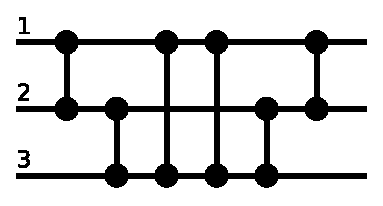
\includegraphics[width=0.4\textwidth]{gates1}
  \hfill
  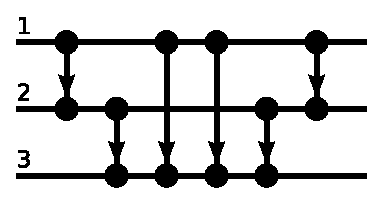
\includegraphics[width=0.4\textwidth]{gates2}
  \caption{Quantum Circuits.
  On the left the gates are represented by two-body symmetric interactions of
  the type $X_iX_j+Y_iY_j$.
  On the right the symmetry is broken with with asymmetric interactions of the
  type $X_iY_j-Y_iX_j$.}
  \label{fig:qcircuit}
\end{figure}

In the top left plot in Fig.~\ref{fig:init1},
the gates of Fig.~\ref{fig:qcircuit} acts on the network with the symmetric
Hamiltonian in eq.~\ref{eq:HS}.
The probability of finding the excitation in node two or three is bounded to
some value below 0.6.
In the top right plot the time reversed Hamiltonian
$H'=R_{z1}(\pi)HR_{z1}(\pi)$~is used and shows exactly the same
probabilities.

On the bottom an antisymmetric Hamiltonian (see eq.~\ref{eq:HA}) is used. 
The antisymmetric interaction is given by the initial symmetric Hamiltonian
where the first spin is rotated by $\pi/2$.
In this case the probabilities of encountering the excitation on node two or
three reach almost one.
Moreover the time symmetry is broken as shown by the fourth panel.

\yo{I would suggest a picture (related to Fig.~\ref{fig:init1}), or an
animation,
for a transition diagram between 3 states
(i.e. 3 points, 6 directed arrows with probabilities).
It would make explicit how does probability "circulate". }

\begin{figure}[p]
  \centering
  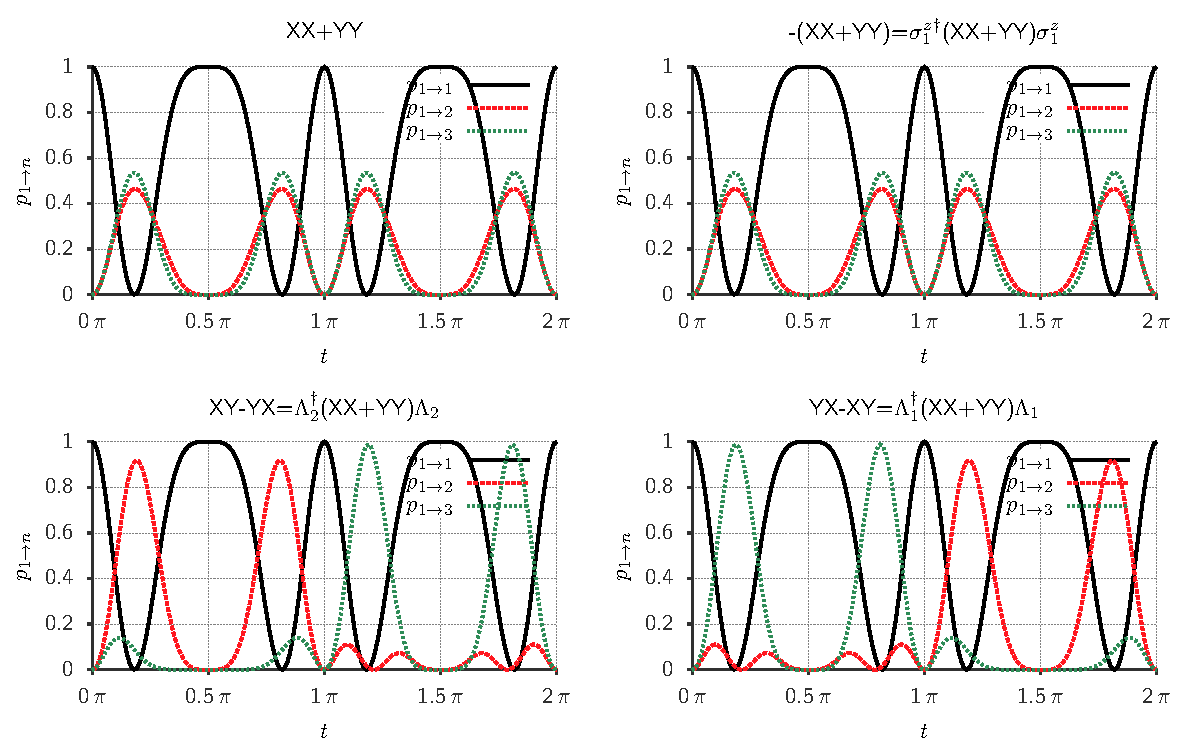
\includegraphics[width=0.8\textwidth]{3qbit_001}
  \caption{Breaking time symmetry.
  The initial state is represented by an excitation on qubit one. The
  occupation probability of qubit $n$ ($p_{1\to n}$) is depicted for different
  type of gates.
  On the top the interaction is symmetric $H=\frac 12 (XX+YY)$. The time inverse
  evolution is simulated rotating the first qubit with $\sigma_z$. The two
  evolutions match.
  The plots on the bottom represent antisymmetric gates $H=XY-YX$. In this
  case the time reversed evolution does not match the positive time one.
  Moreover, breaking time symmetry allows to direct the excitation
  toward the other nodes of the network, reaching an occupation of almost one.
  Here $\Lambda_n$ is the $2\times2$ diagonal matrix with entries 1 and $i$
  acting on the wire $n$.
  }
  \label{fig:init1}
\end{figure}



\begin{figure}[p]
	\begin{center}
		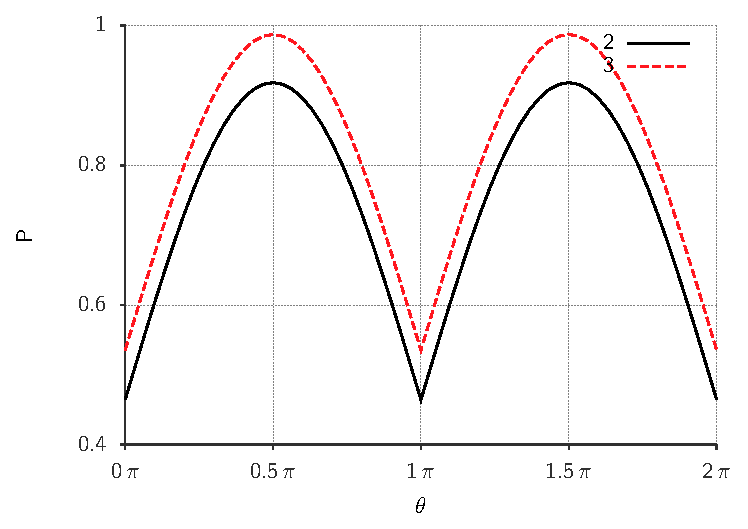
\includegraphics{opt-time}
	\end{center}
	\caption{Optimized Transport for the unitary family $U(\theta)$.
	The plot shows the best value of the transport from site one to site two
	(black solid line) and to site three (red dashed line), optimized on
$t$.}
	\label{fig:opt}
\end{figure}


In Fig.~\ref{fig:init23} the same evolution, with the same gates are shown for
initial states localized on qubit two or three.


\begin{figure}[p]
  \centering
  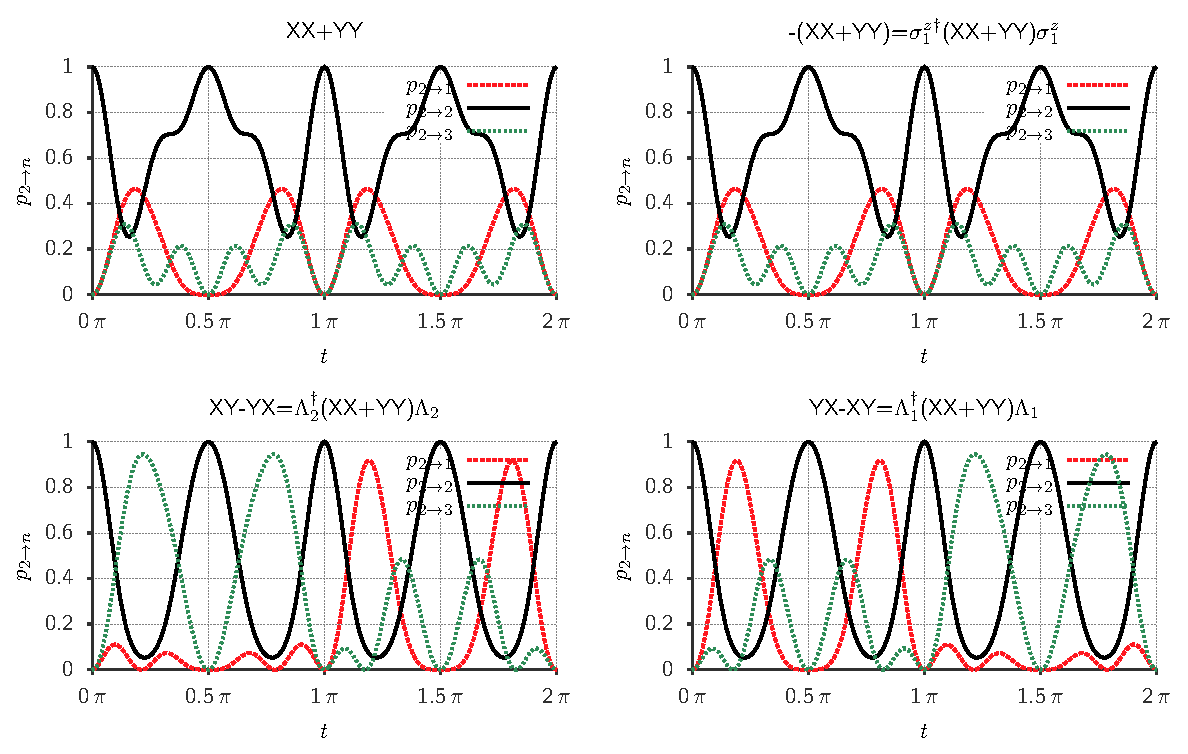
\includegraphics[width=0.8\textwidth]{3qbit_010}\\
  \vskip 10pt
  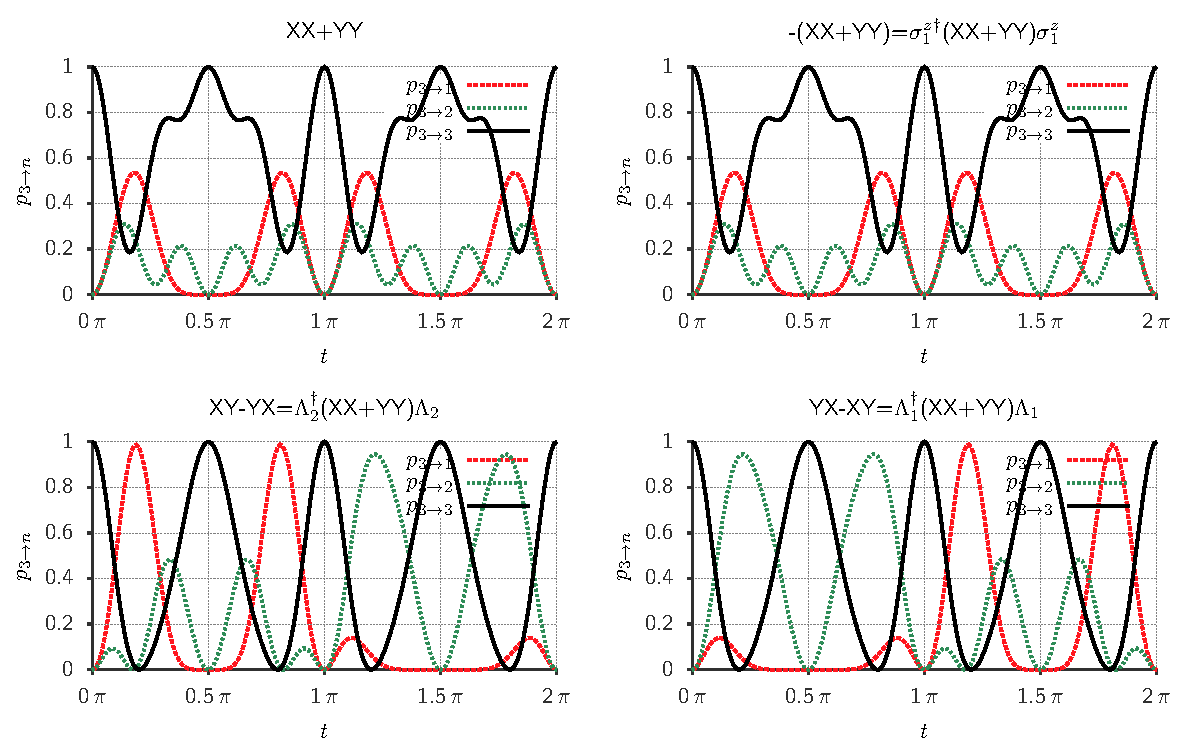
\includegraphics[width=0.8\textwidth]{3qbit_100}
  \caption{Here the initial state is localized on node two or three.}
  \label{fig:init23}
\end{figure}






\section{Probability map} 

\begin{figure}[h]
  \centering
  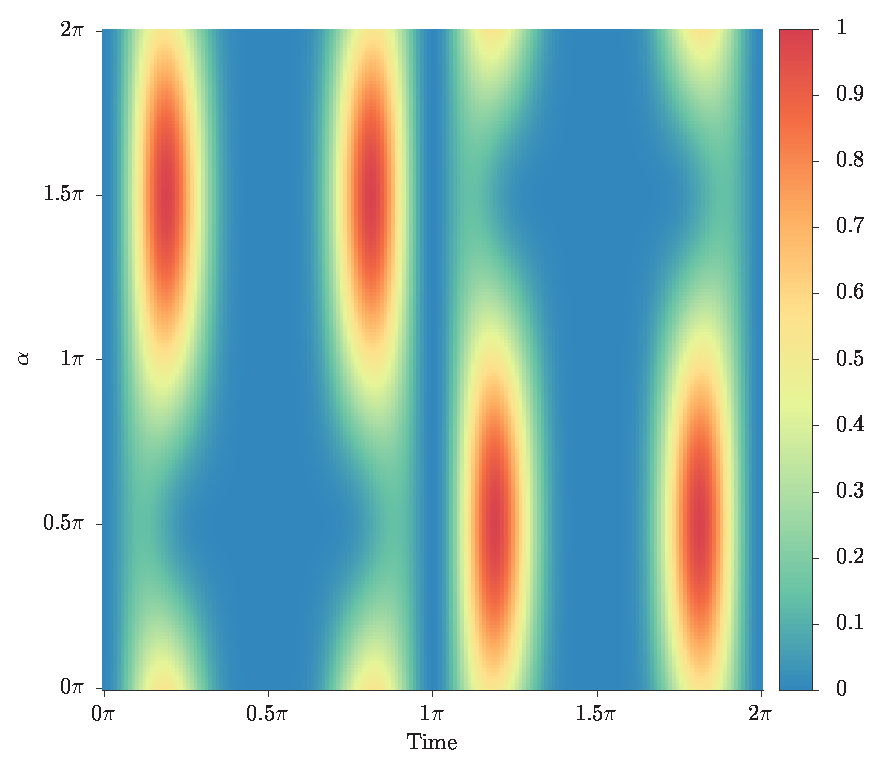
\includegraphics[height=0.4\textwidth]{square}
  \hfill
  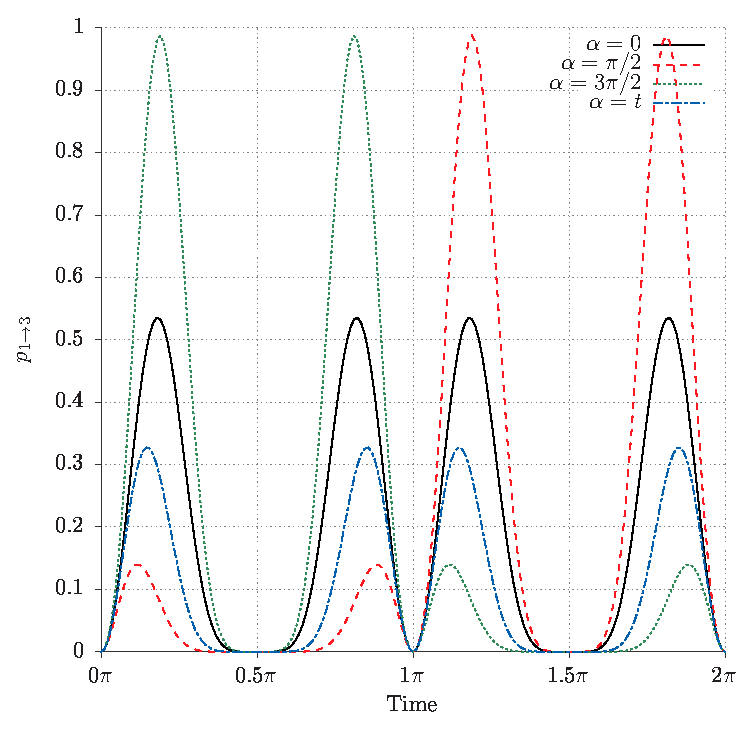
\includegraphics[height=0.4\textwidth]{slices}
  \caption{
    \label{fig:prob}
Probability profiles for several slices in the color map. The probability of
starting from node 1 and at time $t$ with angle $\alpha$ end up on node 3. The
angle $\alpha$ interpolates between
the
two Hamiltonians and the parameter $\theta$ is the time that each gate is
applied.  For $\alpha = 0, n\pi$ the process is necessarily time symmetric. 
The maximum transition probabilities occur when $\alpha = n\pi/2$ in which
case, the Hamiltonian is fully antisymmetric.}  
\end{figure}

We recall now the general definition of the gates we consider here 
\begin{align}
\notag
U_{ij}(\alpha, \theta) = 
Z_i(\alpha)e^{-i\theta(X_iX_j+Y_iY_j)}Z_i^\dagger(\alpha) &= e^{-i
\theta[\cos\alpha(X_iX_j+Y_iY_j)+\sin\alpha(X_iY_j-Y_iX_j)] }
= 
\end{align}

\begin{align}
\begin{pmatrix}
1\\
& \cos(\theta) &  -ie^{-i\alpha}\sin(\theta)\\
& -ie^{i\alpha}\sin(\theta) & \cos(\theta)\\
& & & 1
\end{pmatrix}
\end{align} 

% The circuit we will consider in this experiment is as follows.  
% 
% 
% \begin{figure}[p]
% 	\begin{center}
% %		\includegraphics{}
% 	\end{center}
% 	\caption{TODO: Circuit diagram illustrating also local $Z$ gates (which
% are set to identity for the time-symmetric versions of the experiment). }
% \end{figure}

% \begin{figure}[h]
% 	\begin{center}
% %		\includegraphics{}
% 	\end{center}
% 	\caption{Probability map where the angle $\alpha$ interpolates between
% the
% two Hamiltonians and the parameter $\theta$ is the time that each gate is
% applied.  For $\alpha = 0, n\pi$ the process is necessarily time symmetric. 
% The maximum transition probabilities occur when $\alpha = n\pi/2$ in which
% case, the Hamiltonian is fully antisymmetric.}
% \end{figure}

In the experiment we will probe four horizontal slices of this contour plot.  

\begin{itemize}
 \item[$\alpha = 0$] This probes the time-symmetric case, in which case the
node to node transition probability is bounded by one-half (not in the circuit
version, see the remark below). 
\item[$\alpha = \pi$] This is the dagger of the process where $\alpha = 0$. 
\item[$\alpha = \pi/2$] This illustrates that enhancement is possible (as is
suppression) by breaking time-reversal symmetry. 
\item[$\alpha = 3\pi/2$] This is the dagger of the process where $\alpha =
\pi/2$. 
\end{itemize}


\begin{remark}[Inequivalence of gate model and continuous evolution] 
Note that in the continuous time variant, the probability of the time symmetric
transition is bounded by $1/2$ and when breaking time-reversal symmetry, you
can get perfect transfer.  Interestingly, in the circuit version both of these
statements seem no longer true, as illustrated in Figure~\ref{fig:prob}. 
\end{remark}



\section{Questions}

\begin{enumerate} 
\item other ideas?   
\end{enumerate} 







\bibliography{chiral-bib}

\end{document}

 
